\chapter{Aufgabe 1 - Installation des Betriebssystem}
\section{Cluster-Layout}
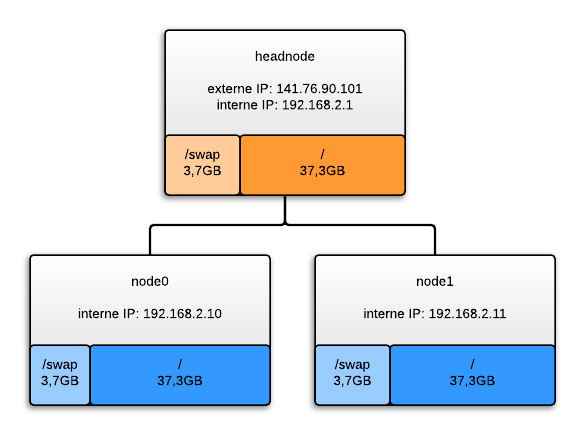
\includegraphics[width=400px]{cluster_layout.png}

/home und /shared werden exportiert.

\section{Betriebssysteminstallation}
\begin{lstlisting}[style=Bash]
# apt-get update 
# apt-get upgrade 
\end{lstlisting}
\begin{lstlisting}[style=Bash]
# adduser --geco GECO <username>
\end{lstlisting}
\begin{lstlisting}[style=Bash]
# apt-get install sudo
\end{lstlisting}
Sudoers-File in /etc/sudoers konfigureren:
(für alle user)
\begin{lstlisting}[style=Bash]
...
<username> ALL=(ALL)NOPASSWD:ALL
...
\end{lstlisting}
\begin{lstlisting}[style=Bash]
$ wget http://lctp.zih.tu-dresden.de/key/<username>.key
$ cat <username>.key >> ~.ssh/authorized_keys
\end{lstlisting}
\begin{lstlisting}[style=Bash]
# passwd -l root 
\end{lstlisting}


\section{SSH-Server}
Install SSH-Server
\begin{lstlisting}[style=Bash]
# apt-get install openssh-server 
\end{lstlisting}


/etc/hosts.allow konfigureren:
\begin{lstlisting}[style=Bash]
...
sshd: 141.76.0.0/255.255.0.0
sshd: 141.30.0.0/255.255.0.0
sshd: 192.168.2.0/255.255.255.0
sshd: LOCAL 
\end{lstlisting}
/etc/hosts.deny konfigureren:
\begin{lstlisting}[style=Bash]
...
sshd: ALL
\end{lstlisting}

SSH-Server in /etc/ssh/sshd\_config konfigureren:
\begin{lstlisting}[style=Bash]
...
PermitRootLogin no
RSAAuthentication yes
PubkeyAuthentication yes
...
AllowUsers *@141.76.*.*
AllowUsers *@141.30.*.*
AllowUsers *@192.168.2.*.*
AllowUsers *@localhost
# SSH server auf den nodes:
UseDNS no
\end{lstlisting}

Für jeden User
\begin{lstlisting}[style=Bash]
$ ssh-keygen -b 1024 -N ''
$ cat ~.ssh/id_rsa.pub >> ~./ssh/authorized_keys
\end{lstlisting}

Ein Sscript zur automatischen Nutzererstellung:
(dazu muss das paket whois installiert sein)
\lstinputlisting[style=Bash]{../aufgabe1/addusers.sh}

\section{Parallel Distributed Shell}
\begin{lstlisting}[style=Bash]
# apt-get install pdsh
\end{lstlisting}
/etc/genders
\begin{lstlisting}[style=Bash]
localhost headnode
node0 computenodes
\end{lstlisting}
~/.ssh/config
\begin{lstlisting}[style=Bash]
StrictHostKeyChecking no
\end{lstlisting}
